\documentclass[spanish]{beamer}

%%% CODIFICACIÓN

%\usepackage[x11names, rgb, html]{xcolor}
\usepackage[utf8]{inputenc}
\usepackage[spanish]{babel}
\usepackage{graphics,tikz}

%%% FUENTES

\usepackage[T1]{fontenc}
%\usepackage[familydefault,regular]{Chivo}
\usepackage{newtxsf} % Fuente de matemáticas
\usepackage[scaled=.85]{FiraMono}

\setbeamertemplate{navigation symbols}{}

%%% COLORES

%% Colores de Solarized

\definecolor{sbase03}{HTML}{002B36}
\definecolor{sbase02}{HTML}{073642}
\definecolor{sbase01}{HTML}{586E75}
\definecolor{sbase00}{HTML}{657B83}
\definecolor{sbase0}{HTML}{839496}
\definecolor{sbase1}{HTML}{93A1A1}
\definecolor{sbase2}{HTML}{EEE8D5}
\definecolor{sbase3}{HTML}{FDF6E3}
\definecolor{syellow}{HTML}{B58900}
\definecolor{sorange}{HTML}{CB4B16}
\definecolor{sred}{HTML}{DC322F}
\definecolor{smagenta}{HTML}{D33682}
\definecolor{sviolet}{HTML}{6C71C4}
\definecolor{sblue}{HTML}{268BD2}
\definecolor{scyan}{HTML}{2AA198}
\definecolor{sgreen}{HTML}{859900}

%% Colores del documento

\definecolor{background}{RGB}{237,237,237}
\definecolor{text}{RGB}{78,78,78}
\definecolor{accent}{RGB}{129, 26, 24}
\definecolor{accent2}{HTML}{814918}
\definecolor{accent3}{HTML}{136618}
\definecolor{accent4}{HTML}{0F4B4E}
\definecolor{accent5}{HTML}{681341}
\definecolor{accent6}{HTML}{1F1B5A}

%%% LISTINGS

\usepackage{listingsutf8}

%% Las tildes

\lstset{
  inputencoding=utf8/latin1
}

%% Colores de Solarized para listings

\lstset{
  % How/what to match
  % sensitive=true,
  language=C++,
  % Border (above and below)
  %frame=lines,
  % Line number
  numbers=left,
  % Extra margin on line (align with paragraph)
  xleftmargin=\parindent,
  % Put extra space under caption
  belowcaptionskip=1\baselineskip,
  % Colors
  % backgroundcolor=\color{sbase3},
  basicstyle=\tiny\ttfamily\color{text},
  keywordstyle=\color{accent3},
  commentstyle=\color{accent5},
  stringstyle=\color{accent2},
  numberstyle=\color{text},
  identifierstyle=\color{accent4},
  % Break long lines into multiple lines?
  breaklines=true,
  % Show a character for spaces?
  showstringspaces=false,
  tabsize=2
}

\setbeamerfont{framesubtitle}{size=\normalfont\tiny}
\setbeamercolor{framesubtitle}{fg=white}


%%% AJUSTES DE BEAMER

% ¿Negrita en el título de diapositiva o no?
%\setbeamertemplate{frametitle}{\color{accent}\vspace*{1cm}\bfseries\insertframetitle\par\vskip-6pt}

\setbeamertemplate{frametitle}{\color{accent}\vspace*{1cm}\insertframetitle\par\vskip-6pt}

\setbeamertemplate{itemize items}[circle] % Viñetas de itemize

%%% CONFIGURACIÓN DE COLORES DE BEAMER

\setbeamercolor{background canvas}{bg=background}
\setbeamercolor{normal text}{fg=text}
\setbeamercolor{alerted text}{fg=accent}
\setbeamercolor{block title}{fg=accent}
\setbeamercolor{alerted text}{fg=accent}
\setbeamercolor{itemize item}{fg=accent}
\setbeamercolor{enumerate item}{fg=accent}
\setbeamercolor*{title}{fg=accent}
\setbeamercolor{qed symbol}{fg=accent}
\usebeamercolor[fg]{normal text}

%%% PGFPLOTSTABLE

\usepackage{pgfplotstable}


\pgfplotstableset{
columns/0/.style={
     column name={Elementos},
   },
columns/1/.style={
     column name={Tiempo en segundos},
   },
}

%%% INFORMACIÓN DEL DOCUMENTO

\title{Algorítmica: práctica 3}
\subtitle{Encontrar un recubrimiento minimal de un grafo}
\author{Sofía Almeida Bruno\\ Antonio Coín Castro\\ María Victoria Granados Pozo\\ Miguel Lentisco Ballesteros\\ José María Martín Luque\\ \vspace{1em}Grupo 2}
\begin{document}


\maketitle

\begin{frame}{Objetivo}
	
	Encontrar un recubrimiento minimal del grafo no dirigido G=(V,E).
	Un conjunto U $\subseteq$ V es un recubrimiento de G si cada arista en E incide en, al menos, un vértice o nodo de U.
	
	La solución que proporcionamos es el conjunto de nodos que forman el recubrimiento junto con el coste (número de nodos). 
\end{frame}

\begin{frame}{Ejemplo}
	\begin{figure}[H]
		\centering 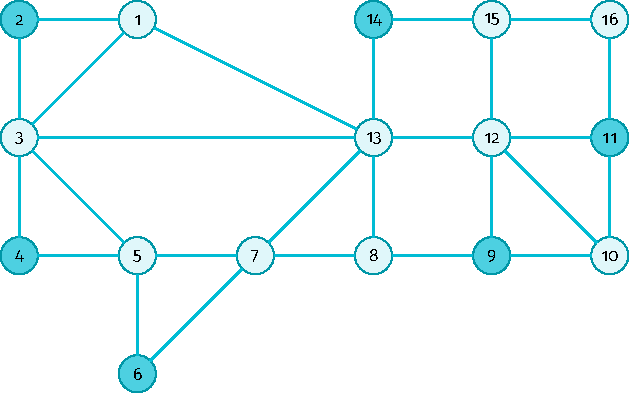
\includegraphics{./img/grafo.pdf}
	\end{figure}
\end{frame}

\begin{frame}{Componentes Greedy}
	\begin{itemize}
		\item \textit{Lista de candidatos:} nodos
		\item \textit{Lista de candidatos utilizados:} nodos considerados
		\item \textit{Función solución:} no haya ninguna arista sin considerar %%o que el vector de incidencias sea 0
		\item \textit{Criterio de factibilidad:} el nodo no está en la lista de candidatos utilizados
		\item \textit{Función objetivo:} recubrimiento de coste mínimo
		\item \textit{Función de selección:} nodo en el que inciden más aristas
		\lstinputlisting[language=C++, linerange={13-25}]{./src/Algoritmo.cpp}
	\end{itemize}
\end{frame}

\begin{frame}{Algoritmo}
	\lstinputlisting[language=C++, linerange={26-40}]{./src/Algoritmo.cpp}
\end{frame}

\begin{frame}{Algoritmo}
	\lstinputlisting[language=C++, linerange={40-60}]{./src/Algoritmo.cpp}
\end{frame}

\begin{frame}{Pseudocódigo}


\end{frame}

\begin{frame}{Ejemplo paso a paso}
	\begin{figure}[H]
		\centering 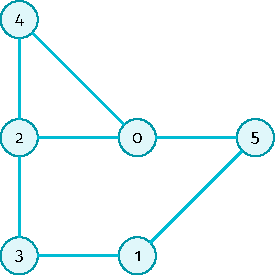
\includegraphics{./img/grafo-ejemplo-sin-recubrir.pdf}
	\end{figure}

\end{frame}

%% FIXME Poner bien la presentación
\begin{frame}{Inicialización}
	N = num\_nodos = 6
	
	M = sol.coste = 0
	
	$$  L = p.matriz\_adyacencia = 
\begin{pmatrix}
  0 & 0 & 1 & 0 & 1 & 1 \\
  0 & 0 & 0 & 1 & 0 & 1 \\
  1 & 0 & 0 & 1 & 1 & 0 \\
  0 & 1 & 1 & 0 & 0 & 0 \\
  1 & 0 & 1 & 0 & 0 & 0 \\
  1 & 1 & 0 & 0 & 0 & 0
\end{pmatrix}$$

	$$  VI = incidencias = 
\begin{pmatrix}
  3 \\
  2 \\
  3 \\
  2 \\
  2 \\
  2
\end{pmatrix}$$

	p = pos\_max = 0
	
\end{frame}

\begin{frame}{Bucle while}
	incidencias[0] = 3 > 0\\
	T = \{0\}\\
	M = sol.coste = 1
	\begin{figure}[H]
		\centering 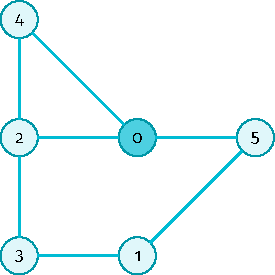
\includegraphics{./img/grafo-ejemplo-1.pdf}
	\end{figure}
\end{frame}

\begin{frame}{}
	$$  VI = incidencias = 
	\begin{pmatrix}
	  3 \\
	  2 \\
	  3 \\
	  2 \\
	  2 \\
	  2
	\end{pmatrix} \implies  VI = incidencias = 
	\begin{pmatrix}	
	  0 \\
	  2 \\
	  2 \\
	  2 \\
	  1 \\
	  1
	\end{pmatrix}$$

	\begin{figure}[H]
		\centering 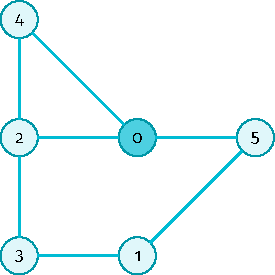
\includegraphics{./img/grafo-ejemplo-1.pdf}
	\end{figure}
	p = pos\_max = 1

\end{frame}

\begin{frame}{Bucle while}
	incidencias[1] = 2 > 0\\
	T = \{0, 1\}\\
	M = sol.coste = 2
	\begin{figure}[H]
		\centering 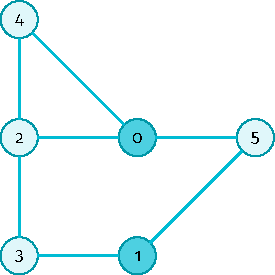
\includegraphics{./img/grafo-ejemplo-2.pdf}
	\end{figure}	
\end{frame}

\begin{frame}{}
	$$  VI = incidencias = 
	\begin{pmatrix}
	  0 \\
	  2 \\
	  2 \\
	  2 \\
	  1 \\
	  1
	\end{pmatrix} \implies  VI = incidencias = 
	\begin{pmatrix}	
	  0 \\
	  0 \\
	  2 \\
	  1 \\
	  1 \\
	  0
	\end{pmatrix}$$
	\begin{figure}[H]
		\centering 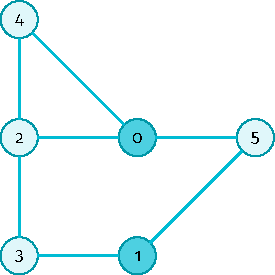
\includegraphics{./img/grafo-ejemplo-2.pdf}
	\end{figure}
\end{frame}

\begin{frame}{Bucle while}
	incidencias[2] = 2 > 0\\
	T = \{0, 1, 2\}\\
	M = sol.coste = 3
	\begin{figure}[H]
		\centering 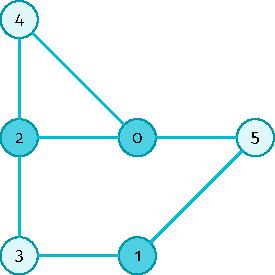
\includegraphics{./img/grafo-ejemplo.pdf}
	\end{figure}
\end{frame}

\begin{frame}{}
	$$  VI = incidencias = 
	\begin{pmatrix}
	  0 \\
	  0 \\
	  2 \\
	  1 \\
	  1 \\
	  0
	\end{pmatrix} \implies  VI = incidencias = 
	\begin{pmatrix}	
	  0 \\
	  0 \\
	  0 \\
	  0 \\
	  0 \\
	  0
	\end{pmatrix}$$
	\begin{figure}[H]
		\centering 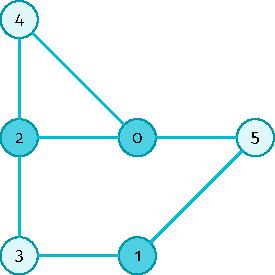
\includegraphics{./img/grafo-ejemplo.pdf}
	\end{figure}
\end{frame}

\begin{frame}{Eficiencia teórica}
    \fontsize{8pt}{7.2}\selectfont
	\begin{center}
	\resizebox*{11cm}{!}{
		%% GNUPLOT: LaTeX picture with Postscript
\begingroup
  \makeatletter
  \providecommand\color[2][]{%
    \GenericError{(gnuplot) \space\space\space\@spaces}{%
      Package color not loaded in conjunction with
      terminal option `colourtext'%
    }{See the gnuplot documentation for explanation.%
    }{Either use 'blacktext' in gnuplot or load the package
      color.sty in LaTeX.}%
    \renewcommand\color[2][]{}%
  }%
  \providecommand\includegraphics[2][]{%
    \GenericError{(gnuplot) \space\space\space\@spaces}{%
      Package graphicx or graphics not loaded%
    }{See the gnuplot documentation for explanation.%
    }{The gnuplot epslatex terminal needs graphicx.sty or graphics.sty.}%
    \renewcommand\includegraphics[2][]{}%
  }%
  \providecommand\rotatebox[2]{#2}%
  \@ifundefined{ifGPcolor}{%
    \newif\ifGPcolor
    \GPcolortrue
  }{}%
  \@ifundefined{ifGPblacktext}{%
    \newif\ifGPblacktext
    \GPblacktextfalse
  }{}%
  % define a \g@addto@macro without @ in the name:
  \let\gplgaddtomacro\g@addto@macro
  % define empty templates for all commands taking text:
  \gdef\gplbacktext{}%
  \gdef\gplfronttext{}%
  \makeatother
  \ifGPblacktext
    % no textcolor at all
    \def\colorrgb#1{}%
    \def\colorgray#1{}%
  \else
    % gray or color?
    \ifGPcolor
      \def\colorrgb#1{\color[rgb]{#1}}%
      \def\colorgray#1{\color[gray]{#1}}%
      \expandafter\def\csname LTw\endcsname{\color{white}}%
      \expandafter\def\csname LTb\endcsname{\color{black}}%
      \expandafter\def\csname LTa\endcsname{\color{black}}%
      \expandafter\def\csname LT0\endcsname{\color[rgb]{1,0,0}}%
      \expandafter\def\csname LT1\endcsname{\color[rgb]{0,1,0}}%
      \expandafter\def\csname LT2\endcsname{\color[rgb]{0,0,1}}%
      \expandafter\def\csname LT3\endcsname{\color[rgb]{1,0,1}}%
      \expandafter\def\csname LT4\endcsname{\color[rgb]{0,1,1}}%
      \expandafter\def\csname LT5\endcsname{\color[rgb]{1,1,0}}%
      \expandafter\def\csname LT6\endcsname{\color[rgb]{0,0,0}}%
      \expandafter\def\csname LT7\endcsname{\color[rgb]{1,0.3,0}}%
      \expandafter\def\csname LT8\endcsname{\color[rgb]{0.5,0.5,0.5}}%
    \else
      % gray
      \def\colorrgb#1{\color{black}}%
      \def\colorgray#1{\color[gray]{#1}}%
      \expandafter\def\csname LTw\endcsname{\color{white}}%
      \expandafter\def\csname LTb\endcsname{\color{black}}%
      \expandafter\def\csname LTa\endcsname{\color{black}}%
      \expandafter\def\csname LT0\endcsname{\color{black}}%
      \expandafter\def\csname LT1\endcsname{\color{black}}%
      \expandafter\def\csname LT2\endcsname{\color{black}}%
      \expandafter\def\csname LT3\endcsname{\color{black}}%
      \expandafter\def\csname LT4\endcsname{\color{black}}%
      \expandafter\def\csname LT5\endcsname{\color{black}}%
      \expandafter\def\csname LT6\endcsname{\color{black}}%
      \expandafter\def\csname LT7\endcsname{\color{black}}%
      \expandafter\def\csname LT8\endcsname{\color{black}}%
    \fi
  \fi
    \setlength{\unitlength}{0.0500bp}%
    \ifx\gptboxheight\undefined%
      \newlength{\gptboxheight}%
      \newlength{\gptboxwidth}%
      \newsavebox{\gptboxtext}%
    \fi%
    \setlength{\fboxrule}{0.5pt}%
    \setlength{\fboxsep}{1pt}%
\begin{picture}(5760.00,4320.00)%
    \gplgaddtomacro\gplbacktext{%
      \colorrgb{0.30,0.30,0.30}%
      \put(1386,1060){\makebox(0,0)[r]{\strut{}$\textcolor{text}{0}$}}%
      \colorrgb{0.30,0.30,0.30}%
      \put(1386,1349){\makebox(0,0)[r]{\strut{}$\textcolor{text}{0.05}$}}%
      \colorrgb{0.30,0.30,0.30}%
      \put(1386,1638){\makebox(0,0)[r]{\strut{}$\textcolor{text}{0.1}$}}%
      \colorrgb{0.30,0.30,0.30}%
      \put(1386,1926){\makebox(0,0)[r]{\strut{}$\textcolor{text}{0.15}$}}%
      \colorrgb{0.30,0.30,0.30}%
      \put(1386,2215){\makebox(0,0)[r]{\strut{}$\textcolor{text}{0.2}$}}%
      \colorrgb{0.30,0.30,0.30}%
      \put(1386,2504){\makebox(0,0)[r]{\strut{}$\textcolor{text}{0.25}$}}%
      \colorrgb{0.30,0.30,0.30}%
      \put(1386,2793){\makebox(0,0)[r]{\strut{}$\textcolor{text}{0.3}$}}%
      \colorrgb{0.30,0.30,0.30}%
      \put(1386,3081){\makebox(0,0)[r]{\strut{}$\textcolor{text}{0.35}$}}%
      \colorrgb{0.30,0.30,0.30}%
      \put(1386,3370){\makebox(0,0)[r]{\strut{}$\textcolor{text}{0.4}$}}%
      \colorrgb{0.30,0.30,0.30}%
      \put(1386,3659){\makebox(0,0)[r]{\strut{}$\textcolor{text}{0.45}$}}%
      \colorrgb{0.30,0.30,0.30}%
      \put(1518,928){\rotatebox{45}{\makebox(0,0)[r]{\strut{}$\textcolor{text}{0}$}}}%
      \colorrgb{0.30,0.30,0.30}%
      \put(1903,928){\rotatebox{45}{\makebox(0,0)[r]{\strut{}$\textcolor{text}{500}$}}}%
      \colorrgb{0.30,0.30,0.30}%
      \put(2287,928){\rotatebox{45}{\makebox(0,0)[r]{\strut{}$\textcolor{text}{1000}$}}}%
      \colorrgb{0.30,0.30,0.30}%
      \put(2672,928){\rotatebox{45}{\makebox(0,0)[r]{\strut{}$\textcolor{text}{1500}$}}}%
      \colorrgb{0.30,0.30,0.30}%
      \put(3056,928){\rotatebox{45}{\makebox(0,0)[r]{\strut{}$\textcolor{text}{2000}$}}}%
      \colorrgb{0.30,0.30,0.30}%
      \put(3441,928){\rotatebox{45}{\makebox(0,0)[r]{\strut{}$\textcolor{text}{2500}$}}}%
      \colorrgb{0.30,0.30,0.30}%
      \put(3825,928){\rotatebox{45}{\makebox(0,0)[r]{\strut{}$\textcolor{text}{3000}$}}}%
      \colorrgb{0.30,0.30,0.30}%
      \put(4210,928){\rotatebox{45}{\makebox(0,0)[r]{\strut{}$\textcolor{text}{3500}$}}}%
      \colorrgb{0.30,0.30,0.30}%
      \put(4594,928){\rotatebox{45}{\makebox(0,0)[r]{\strut{}$\textcolor{text}{4000}$}}}%
      \colorrgb{0.30,0.30,0.30}%
      \put(4979,928){\rotatebox{45}{\makebox(0,0)[r]{\strut{}$\textcolor{text}{4500}$}}}%
      \colorrgb{0.30,0.30,0.30}%
      \put(5363,928){\rotatebox{45}{\makebox(0,0)[r]{\strut{}$\textcolor{text}{5000}$}}}%
    }%
    \gplgaddtomacro\gplfronttext{%
      \colorrgb{0.30,0.30,0.30}%
      \put(220,2359){\rotatebox{-270}{\makebox(0,0){\strut{}Tiempo de ejecución (s)}}}%
      \colorrgb{0.30,0.30,0.30}%
      \put(3440,220){\makebox(0,0){\strut{}Tamaño del vector (elementos)}}%
      \colorrgb{0.30,0.30,0.30}%
      \put(3440,3989){\makebox(0,0){\strut{}Ajuste algoritmo clásico}}%
      \csname LTb\endcsname%
      \put(4376,3486){\makebox(0,0)[r]{\strut{}3.22e-09$x^2$+-3.73e-06$x$+2.57e-03}}%
      \csname LTb\endcsname%
      \put(4376,3266){\makebox(0,0)[r]{\strut{}Clásico}}%
    }%
    \gplbacktext
    \put(0,0){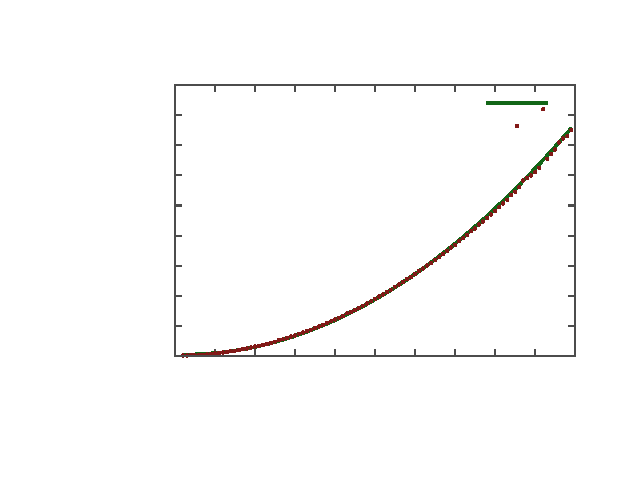
\includegraphics{./graficos/ajuste-clasico}}%
    \gplfronttext
  \end{picture}%
\endgroup

	}
	\end{center}    
\end{frame}



\end{document}

